\documentclass[12 pt, a4paper]{article}
\usepackage[english]{babel}  								% For norsk oppsett
\usepackage[utf8]{inputenc}
\usepackage{amsmath}
\usepackage{amssymb}
\usepackage{graphicx}
\usepackage{tabularx}
\usepackage{tabulary}
\usepackage{subcaption}
\usepackage{hyperref}
\usepackage{fancyhdr}
\usepackage{enumerate}
\usepackage{float}
\usepackage{tikz}
\usepackage{fancyhdr}
\usepackage{lastpage}
\usepackage{circuitikz}
\usepackage{physics}
\usepackage[includeheadfoot, margin =0.5 in]{geometry}
\usepackage[FYS, OnlyFrontpage]{mnfrontpage} 			%SKIFT HER!!!
\usepackage[version=3]{mhchem}
\usepackage{biblatex}%,style=numeric-comp
%\usepackage{cite}
\usepackage{siunitx}
\usepackage{todonotes}
\usepackage{xcolor}
\usepackage{listings}
%%%%
\usepackage[bottom]{footmisc}
\renewcommand\footnoterule{\rule{\linewidth}{0.5pt}}
%\renewcommand[\footnoterule]{%
%	\kern -3pt
%	\hrule width \textwidth height 1pt 
%	\kern 2pt
%}
%%%%
\lstset{basicstyle=\ttfamily,
  showstringspaces=false,
  commentstyle=\color{red},
  keywordstyle=\color{blue}
}
%\usepackage{showframe}  %Dette viser hvordan strukturen på sidene er



\newcommand{\gray}[1]{\textcolor{gray}{#1}}
\newcommand{\spin}[1]{\ifthenelse{#1 = 1}{\uparrow}{\downarrow}}
\newcommand{\tilstand}[4]{
    \(\displaystyle
        \begin{matrix}
			
			\spin{#1}  & \spin{#2}\\
			\spin{#3} & \spin{#4}
			
        \end{matrix}
    \)
}




\setlength{\parindent}{0cm}

\author{
\href{https://scontent.fosl1-1.fna.fbcdn.net/v/t31.0-8/12671762_10153383742266712_8474119290530634136_o.jpg?oh=22ee31dac1e3bff8a581f96848315dbc&oe=5A7942F3}{Erik Skaar}
}



\bibliography{kilder.bib}






\font\myfont=cmr12 at 35pt
\title{\textbf{{\myfont Studies of phase transitions in magnetic systems}}}
\begin{document}
\mnfrontpage
%https://www.flickr.com/photos/knol/2641484620/


\pagestyle{fancy}
\fancyhf{}
\rhead{\href{http://www.uio.no/studier/emner/matnat/fys/FYS3150/index-eng.html}{FYS4150}}
\lhead{\href{https://github.com/erikfsk/Project-4}{Erik Skaar}}
\fancyfoot[CE,LO]{\leftmark}
\fancyfoot[LE,RO]{Page \number\value{page} of \pageref{LastPage}}

\renewcommand{\headrulewidth}{2pt}
\renewcommand{\footrulewidth}{1pt}

\tableofcontents

\pagebreak
\section*{Abstract}%1
Phase transition for a two dimensional magnetic system was studied using the Ising model and the Metropolis algorithm. The Program was confirmed to work by the analytical result of a 2x2 matrix. For stability and convergence a 20x20 lattice was used. The critical temperature $T_C$ for a infinite was approximated through simualations of many different lattices. $T_C$ was approximated to 2.2699\footnote{See table \ref{tab:t-c}}, which is close to the analytical prediction of Lars Onsager.\cite{onsager} 


\section{Introduction}
These laws are not enough to solve the motion of the planets. From the laws one can derive differential equations for the motion, which are not trivial or even possible to solve analytically. This is where computational methods are useful. With the tools developed in computtational physics we can make a prediction to the motion of the planets in our solar system.\footnote{\href{http://www.uio.no/studier/emner/matnat/fys/FYS3150/h17/index.html}{\color{blue}{Semester page for FYS3150 - Autumn 2017}}.} And because of our assignment we kind of have to do this to pass the course.\cite{project4}



\pagebreak
\section{Theory}\label{sec:theory}

\subsection{the Ising model}

The Ising model describes a coupled system. Where only the nearest neighbor affect each other. In this report the Ising model will be applied to a two dimensional magnetic system. This will be a grid of spins, where each spin $s_i$ can either have 1 or 0 as value. The total energy is expressed as: 


\begin{align*}
	E = - \sum_{<i,j>} J_{i,j} s_i s_j
\end{align*}

Where the symbol < kl > indicates that we sum over nearest neighbors only.
If we assume that each coupling has the same magnitude J, then the energy is expressed as: 

\begin{align}
	E = - J \sum_{<i,j>} s_i s_j
	\label{eq:ising-energy}
\end{align}

\subsubsection{Periodic boundary conditions}

When working with a finite matrix we run into a problem with the boundaries. They are missing neighbours. We solve this by introducing periodic boundary conditions. This means that the right neighbour for $S_n$ is assumed to take the value of $S_1$. 

\subsection{Statistical physics}

\subsubsection{the partition function}\label{sec:z-func}

Boltzmann distrubtion is used as the probability distrubtion. Boltzmann distribution states the probability for $E_i$ is proportional to $e^{-\beta E_i}$ , where $\beta$ is $\frac{1}{k_BT}$. k is the boltzmann constant. For this to be a probability distribution, it needs to be normalized. To normalize the distribution divide the sum of probabilities by a constant Z: 

\begin{align*}
	1 = \frac{\sum_{i} e^{-\beta E_i}}{Z}
	\\
	Z = \sum_{i} e^{-\beta E_i}
\end{align*}

Z is called the partition function. 

\subsubsection{Calculation of values}

The partition function is very useful. In combination with the boltzmann distrubution we get a expression for the probability. 

\begin{align*}
	P(E_i) = \frac{e^{-\beta E_i}}{Z}
\end{align*}

For finding a mean value, one can simply make a sum over $P(E_i)$ multiplied by the value of interest. For instance the mean energy is given by: 

\begin{align*}
	\langle E \rangle = \sum_i E_i P(E_i)
\end{align*}

Expressions for important expectation values can be derived such for the energy E, magnetic moment |M|, specific heat capacity $C_v$ and the sesceptibility $\chi$. The expressions used in this report are listed below\cite{compphys}:

\begin{align*}

\end{align*}

\subsubsection{the mean magnetic moment |M|}

\subsubsection{the specific heat $C_V$}

\subsubsection{the susceptibility $\chi$}






















\pagebreak
\section{Method}

\subsection{Metropolis algorithm}\label{sec:metro}

The metropolis algorithm only has a few steps. First, pick one site in the matrix of spins. This process need to be random. For that site, calculate the energy difference if the spin is flipped. Then the algorithm decide whether to flip the spin or not. This is decided based on the energy difference. If the difference is negative flip, then flip the spin. If not, then pick a random number between 0 and 1 and if this number is less then $e^{-\beta \Delta E}$ flip the spin. Else keep the spin. Finally update expectation values.


\subsubsection{Precalculate}

The energy difference is expressed as an exponential function. Exponential values are expensive to calculate. In two dimensions there is a finite number of energy differences. We can precalculated the exponentials. By calculating these in advance the program will run more efficient. It can be shown that the energy difference then is\cite{compphys}:

\begin{align*}
	\Delta E = 2J s_j \sum_{<k>} s_k
\end{align*}


%\subsection{Randomness}

%\todo{REF hvilken random generater bruker vi.}



\pagebreak
\section{Implementation}


The metropolis algorithm was implemented as discussed in section \ref{sec:metro} in the programs called main-"...".cpp. Their is a few different versions of the main.cpp. The only difference is basicly how they write to file. All of the programs discussed in this section can be found at \href{https://github.com/erikfsk/Project-4/tree/master/Project4}{\color{blue}{github}}.
\\
\\
These calculations are expensive in terms of FLOPs. That is why a parallelized version has been made. Not all the code needs to be parallelized. Most of the code in the parallelized version is the same as for the non-parallelized. Except each thread open a specific file for that thread and runs the metropolis algorithm for $\frac{1}{\text{nr. of temperatures}}$. What temperature that each thread calculate is determined by the rank of the thread. Since the rank is a unique number for each thread, all the temperatures calculated is unique from the other temperatures. 
\\
\\
MPI is used since it is easy to implement and it does not have shared memory. The parallelized version should be (nr. of threads - 1) times faster then the normal version.

\begin{center}
\label{tab:parallell}
\captionof{table}{The grids ran for 50'000 Monte Carlo cycles. The test ran on a macbook pro 13. It has a dual core CPU. Expected difference is 2. }
\begin{tabularx}{\textwidth}{c X c X c X c X c}
    \hline 
    \hline 
        Size && Normal && MPI && Expected difference && Actual difference\\ 
    \hline
        40x40   	&&      15.251s	&&		5.991 s 	&&	2.000	&&	2.546	\\  
        60x60   	&&      33.923s	&&		13.351 s	&&	2.000	&&	2.541	\\
        100x100   	&&      92.584s	&&		36.245 s	&&	2.000	&&	2.554	\\
    \hline
\end{tabularx}
\end{center}

The difference was higher, then expected. This is due to the Hyper-Threading technology in this CPU \footnote{\href{https://www.intel.com/content/www/us/en/architecture-and-technology/hyper-threading/hyper-threading-technology.html}{\color{blue}{Intel Hyper-Threading Technology}}}. 
\\
\\
For size scaling we expect a time increased proportional to the size increase squared. 

\begin{center}
\label{tab:expected-time}
\captionof{table}{The table shows how we expect the time to develop and how it actually it develops. There is a minor difference from expected and calculated and that comes from the fact that the program does more then just the algorithm and the fact that the algorithm has not been perfectly implemented.}
\begin{tabularx}{\textwidth}{c X c X c X c}
    \hline 
    \hline 
        Size && Expected time && Actual time && $\frac{T_{i}}{T_{40}}$\\ 
    \hline
        40x40   	&&      x		&&		8.490 s 	&&	1.000	\\  
        60x60   	&&      2.25x	&&		19.350 s	&&	2.279	\\
        100x100   	&&      6.25x	&&		54.068 s	&&	6.368	\\
    \hline
\end{tabularx}
\end{center}






\pagebreak
\section{Result \& Discussion}
\subsection{Analytic 2x2}


\subsubsection{Microstates 2x2}

\begin{center}
\label{tab:states-2x2}
\captionof{table}{This shows the different microstates that is possible for a 2x2 spinmatrix. It also states the energy and magnetic moment for each microstate.}
\begin{tabularx}{\textwidth}{c c c X c c c}
    \hline 
    \hline 
        State & Energy & Magnetic moment && State & Energy & Magnetic moment \\ 
    \hline
        \tilstand{1}{1}{1}{1} & -8J & 4 && \tilstand{0}{0}{0}{0} & -8J & -4 \\ \\
        
        \tilstand{0}{1}{1}{1} & 0J & 2 && \tilstand{1}{0}{0}{0} & 0J & -2 \\ \\
        \tilstand{1}{0}{1}{1} & 0J & 2 && \tilstand{0}{1}{0}{0} & 0J & -2 \\ \\
        \tilstand{1}{1}{0}{1} & 0J & 2 && \tilstand{0}{0}{1}{0} & 0J & -2 \\ \\
        \tilstand{1}{1}{1}{0} & 0J & 2 && \tilstand{0}{0}{0}{1} & 0J & -2 \\ \\

        \tilstand{0}{0}{1}{1} & 0J & 0 && \tilstand{1}{1}{0}{0} & 0J & 0 \\ \\ 
        \tilstand{0}{1}{0}{1} & 0J & 0 && \tilstand{1}{0}{1}{0} & 0J & 0 \\ \\
        \tilstand{1}{0}{0}{1} & 8J & 0 && \tilstand{0}{1}{1}{0} & 8J & 0 \\ \\
    \hline
\end{tabularx}
\end{center}



\begin{center}
\label{tab:states-2x2-summary}
\captionof{table}{The table shows a summary from table \ref{tab:states-2x2}. }
\begin{tabularx}{\textwidth}{c X c X c X c}
    \hline 
    \hline 
        Number of $\color{red}{\uparrow}$ && Multiplicity && Energy && Magnetic moment \\ 
    \hline
        4   &&      1      &&      -8J     &&       4       \\  
        3   &&      4      &&      0J      &&       2       \\
        2   &&      2      &&      8J      &&       0       \\
        2   &&      4      &&      0J      &&       0       \\
        1   &&      4      &&      0J      &&       -2      \\
        0   &&      1      &&      -8J     &&       -4      \\
    \hline
\end{tabularx}
\end{center}












\pagebreak
\subsubsection{Quantities}

We will use the equations from section \ref{sec:expect}.
\\
\\
For energy the eq. \ref{eq:E} will result in:

\begin{align*}
    &Z = \sum_i = e^{-\beta E_i}
    \\
    &\text{T = kT/J = 1} 
    \\
    &Z = \sum_i = e^{-\beta E_i} = 2e^{8} + 2e^{-8} + 12
\end{align*}


For energy the eq. \ref{eq:E} will give the result:

\begin{align*}
    &\langle E \rangle = \sum_i E_iP(E_i)
    \\
    &\text{T = kT/J = 1} 
    \\
    &\langle E \rangle = \frac{1}{Z} \sum_i E_i e^{-E_i}
    \\
    &\langle E \rangle = \frac{1}{Z} \left( 16 e^8 - 16e^{-8} \right) = 7.9839
    \\ 
    &\langle E \rangle /N= \frac{\langle E \rangle}{4} = 1.9959
\end{align*}


For energy the eq. \ref{eq:M} will give the result:

\begin{align*}
    &\langle |M| \rangle = \sum_i M_iP(E_i)
    \\
    &\text{T = kT/J = 1} 
    \\
    &\langle |M| \rangle = \frac{1}{Z} \sum_i M_i e^{-E_i}
    \\
    &\langle |M| \rangle 
    = 
    \frac{1}{Z} 
    \left(
      4\cdot1e^{8} 
    + 2\cdot4e^{0} 
    + 0\cdot2e^{-8} 
    + 0\cdot4e^{0} 
    + 2\cdot4e^{0}  
    + 4\cdot1e^{8}
    \right) 
    \\
    &\langle |M| \rangle 
    = 
    \frac{1}{Z} 
    \left(
    16
    + 8 e^{8}
    \right) = 3.9946
    \\ 
    &\langle |M| \rangle /N= \frac{\langle M \rangle}{4} = 0.9986
\end{align*}

For $C_V$ we need to calculate $\langle E^2 \rangle$:

\begin{align*}
    &\langle E^2 \rangle = \sum_i E_iP(E_i)
    \\
    &\text{T = kT/J = 1} 
    \\
    &\langle E^2 \rangle = \frac{1}{Z} \sum_i E_i^2 e^{-E_i}
    \\
    &\langle E^2 \rangle = \frac{1}{Z} \left( 128 e^8 + 128 e^{-8} \right)
    \\
    &C_V = \langle E^2 \rangle - \langle E \rangle^2 = 0.12832
    \\ 
    &C_V/N = 0.03208
\end{align*}



For $\chi$ we need to calculate $\langle M^2 \rangle$:

\begin{align*}
    &\langle M^2 \rangle = \sum_i M_i^2P(E_i)
    \\
    &\text{T = kT/J = 1} 
    \\
    &\langle M^2 \rangle = \frac{1}{Z} \sum_i M_i^2 e^{-E_i}
    \\
    &\langle M^2 \rangle 
    = 
    \frac{1}{Z} 
    \left(
      16\cdot1e^{8} 
    + 4\cdot4e^{0} 
    + 0\cdot2e^{-8} 
    + 0\cdot4e^{0} 
    + 4\cdot4e^{0}  
    + 16\cdot1e^{8}
    \right) 
    \\
    &\langle M^2 \rangle 
    = 
    \frac{1}{Z} 
    \left(
    32
    + 32 e^{8}
    \right) = 15.9732
    \\
    &\text{$\langle M \rangle$ is 0 which makes $\langle \chi \rangle = \langle M^2 \rangle$}
    \\
    &\langle \chi \rangle = 15.9732
    \\
    &\langle \chi \rangle / N = 3.9933
\end{align*}

Below you can see a summary for the quantities:

\begin{align*}
    \langle E \rangle /N &= 1.9959  \qquad &&\langle |M| \rangle /N = 0.9986
    \\
    C_V/N &= 0.03208  \qquad &&\langle \chi \rangle / N = 0.004010
\end{align*}









\pagebreak
\subsection{example}

\begin{figure}[H]
    \centering
    \begin{subfigure}{0.5\textwidth}
        \centering
        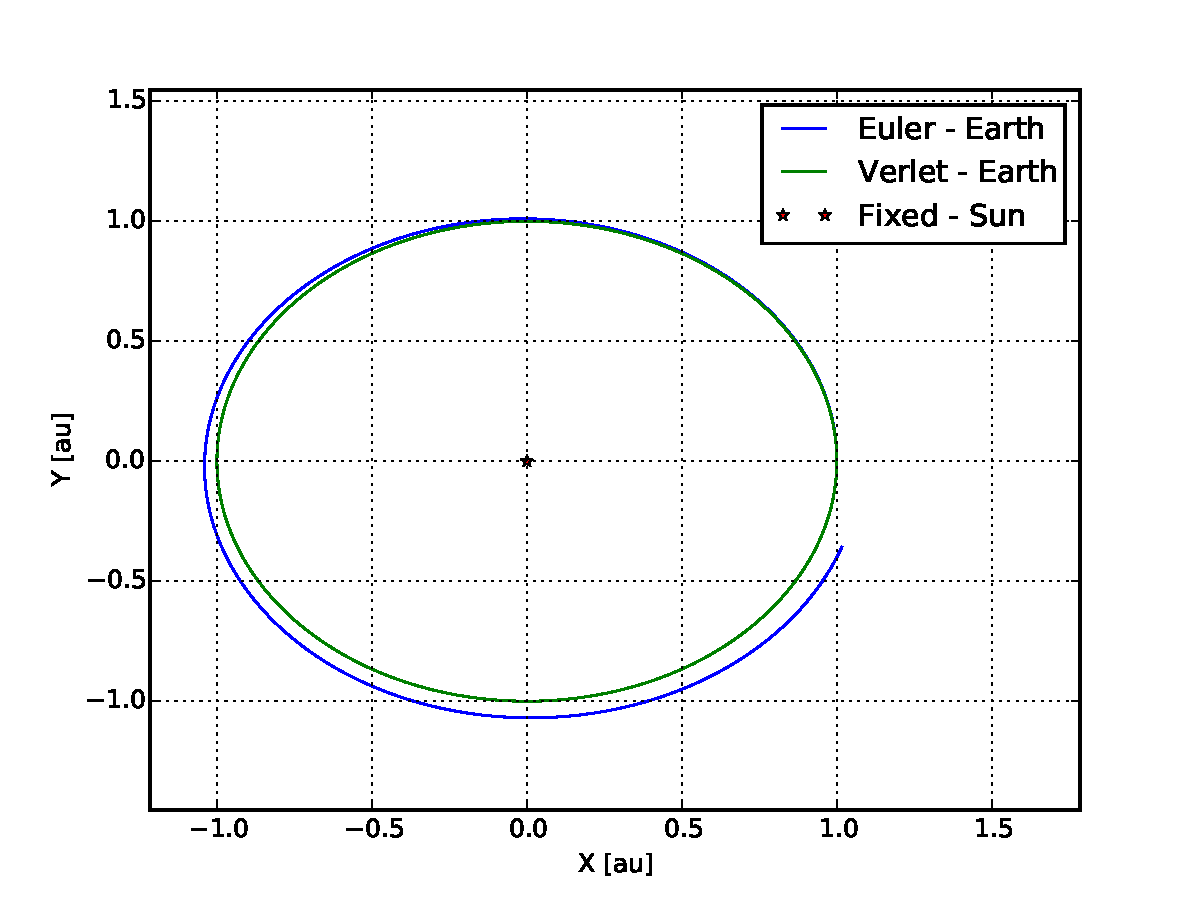
\includegraphics[width=\linewidth]{result/bilder/earth-sun.pdf}
    	\caption{}
    \end{subfigure}%
    ~ 
    \begin{subfigure}{0.5\textwidth}
        \centering
        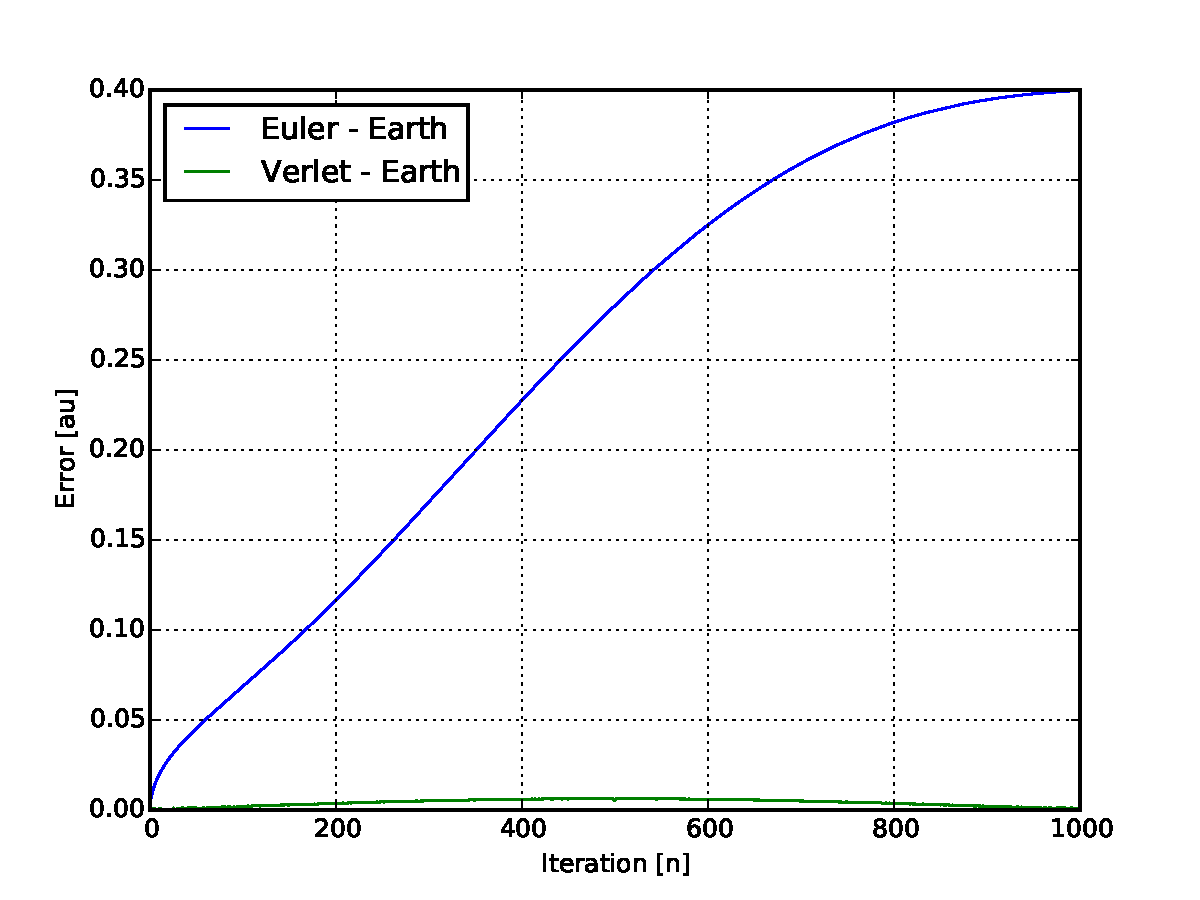
\includegraphics[width=\linewidth]{result/bilder/earth-sun-error.pdf}
        \caption{}
    \end{subfigure}
    \caption{a) shows the orbit of earth around the sun. The intial velocity is set to $2\pi$ in y direction and the start position to 1 au in x direction. b) shows how the error develops. The intial values should give a perfect circular motion. So the error is calculated by $r_i - r_{0}$. It is apparent that the Verlet-Velocity method is a better approximation. This simulation was with 1000 points with the end time of 1 year. Both simulations was produced by \href{https://github.com/erikfsk/Project-3/tree/master/Project3/earth-sun-standard-results}{\textcolor{blue}{plot\_earth\_sun.py}}}
    \label{fig:earth-sun}
\end{figure}




%\pagebreak
%\section{Discussion}
%\input{discussion/discussion}

\pagebreak
\section{Conclusion}
The program has been tested with the analytical solution for a 2x2 grid of spins. A 20x20 matrix was tested for convergence. The convergence result was used for future calculations. For finding $T_C$ extrapolation and equation \ref{eq:t-c} was used on the dataset from 20,60,100,140 and 200 lattices. \footnote{Assignment asked for 40,60,100 and 140. I toke the liberty to use a different set of L values and a different T interval.} From the equation the best result was 2.699 and from extrapolation 2.261 was obtained. From literature the exact result is known as approximatively 2.269.\cite{onsager}  
\\
\\
For future work one should calculate more exact values of the transition states for the finite lattices. This takes a lot of computational power, but will in exchange yield a better result.\footnote{Hopefully}
\\
\\
For further information and more results can be found at my github. Most of what has been discussed in this report has extra figures and datasets there. 
\\
\\
\\
\\
\\
\\
\\
\\
\\
\\
\\
\\
\\
\\
\\
\\
\\
\\
\\
\\
\\
\\
\\
\\
\printbibliography


% \section{Appendix}\label{sec:appendix}
% \begin{lstlisting}[language=c++]
//FLOPs FOR ACCELERATION
// 1 FLOP * 3 directions
dx = x1 - x2
// 3 FLOPs
r = sqrt(dx*dx + dy*dy + dz*dz)
// 7 FLOPs
a = - (Gconst*m*M/(r*r)) / (m*r)
// 2 FLOPs * 3 directions
a = a + a*(x1-x2);																	
//TOTAL FLOPs = 19 FLOPs 


//FLOPs FOR POSITION :: EULER
// 2 FLOPs * 3 directions
x = x + t_step*Vx															
//TOTAL FLOPs = 6 FLOPs 


//FLOPs FOR VELOCITY :: EULER
// 2 FLOPs * 3 directions
Vx = Vx + t_step*ax															
//TOTAL FLOPs = 6 FLOPs 


//FLOPs FOR POSITION :: Verlet
// 6 FLOPs * 3 directions
x = x + t_step*Vx + (0.5*t_step*t_step*a);
//TOTAL FLOPs = 21 FLOPs


//FLOPs FOR VELOCITY :: Verlet
// 4 FLOPs * 3 directions
Vx = Vx + (0.5*t_step*(Ax+Ax_old));
//TOTAL FLOPs = 12 FLOPs
\end{lstlisting}

\pagebreak

\begin{figure}[H]
		\centering
		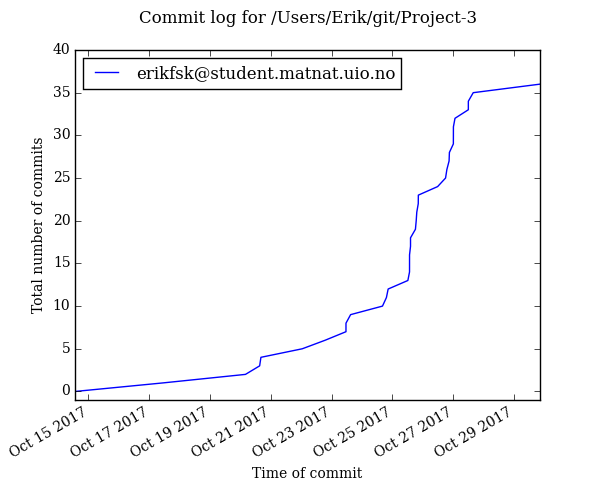
\includegraphics[width=0.7\linewidth]{appendix/bilder/workflow.png}
		\caption{Our retarded workflow... Next time maybe it will be better?}
		\label{fig:ab}
\end{figure}



%\begin{align*}
%&n \qquad &2^n - (-1)^n\\
%&n+1 \qquad &2^{n+1} - (-1)^{n+1} \\
%& &= 2(2^{n}) - (-1)^{n+1}\\
%& &= 2(2^{n} + (-1)^n  + (-1)^{n+1}) - (-1)^{n+1}\\
%& &= 2(2^{n} + (-1)^n  - (-1)^{n}) - (-1)^{n+1}\\
%& &= 2(2^{n}- (-1)^{n}) + 2(-1)^n  + (-1)^{n}\\
%& &= 2(2^{n}- (-1)^{n}) + 3(-1)^n \\
%\end{align*}



%\begin{tabular}{|c|c|c|c|c|c|c|}
%	\hline 
%	n & General & Specific & LU & fastest & slowest & $\frac{slowest}{fastest}$\\ 
%	\hline
%	10 & 6.5e-05 & 5e-06 & 4e-05 & Specific & General & 13.0\\ 
%	\hline 
%	100 & 7.5e-05 & 8e-06 & 0.0023 & Specific & LU & 287.5\\ 
%	\hline 
%	1000 & 0.00014 & 4e-05 & 0.26 & Specific & LU & 6500\\ 
%	\hline
%	10000 & 0.0007 & 0.0005 & 142.5 & Specific & LU & 285000 \\ 
%	\hline
%\end{tabular}

%\begin{figure}[H]
%		\centering
%		\includegraphics[width=0.7\linewidth]{ab.png}
%		\caption{Atomene er gule kuler, de elementære vektorene er blå og a vektorene er grønne.}
%		\label{fig:ab}
%\end{figure}



\end{document}
